\documentclass{standalone}

\usepackage[dvipsnames]{xcolor}
\usepackage{tikz}

\usepackage{booktabs}

\usepackage{fontspec}
\setmainfont{Tex Gyre Schola}

\usepackage{array}
%\renewcommand{\arraystretch}{2}
\begin{document}

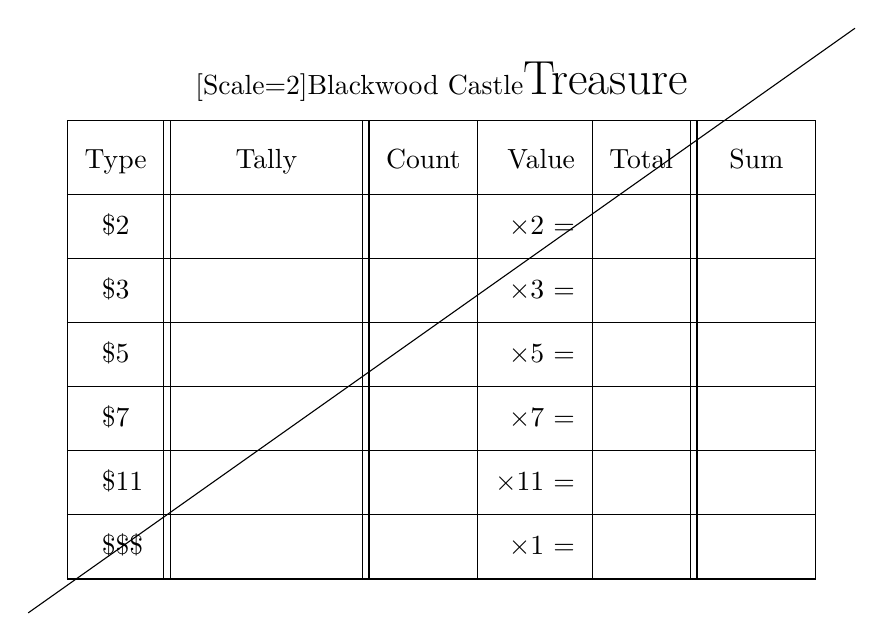
\begin{tikzpicture}

%\path[draw] (-52.5mm,-74.25mm) -- (52.5mm, 74.25mm);
\path[draw] (-52.5mm, -37.125mm) -- (52.5mm, 37.125mm);

\node at (0,0) {
\begin{tabular}{|c||m{20mm}||c|r|c||c|}%||rrrrrl|l|}
\multicolumn{6}{c}{\setmainfont[Scale=2]{Blackwood Castle}\LARGE Treasure} \\[2mm]\hline
Type\raisebox{-3mm}{\rule{0mm}{9mm}} & \centering Tally & Count & \centering Value & Total & \phantom{S}Sum\phantom{S}\\[2mm]\hline % & 2 & 3 & 5 & 7 & 11 & Bonus & Total \\\hline
\$2\raisebox{-3mm}{\rule{0mm}{8mm}} & & & \raggedleft \times 2 = & & \\\hline
\$3\raisebox{-3mm}{\rule{0mm}{8mm}} & & & \raggedleft \times 3 = & & \\\hline
\$5\raisebox{-3mm}{\rule{0mm}{8mm}} & & & \raggedleft \times 5 = & & \\\hline
\$7\raisebox{-3mm}{\rule{0mm}{8mm}} & & & \raggedleft \times 7 = & & \\\hline
\phantom{1}\$11\raisebox{-3mm}{\rule{0mm}{8mm}} & & & \raggedleft \times 11 = & & \\\hline
\phantom{\$}\$\$\$\raisebox{-3mm}{\rule{0mm}{8mm}} & & & \raggedleft \times 1 = & & \\\hline%% & & & & & & &\\
\end{tabular}
};
\end{tikzpicture}
\end{document}